\begin{figure}[htbp]
  \centering
  \begin{minipage}[t]{0.57\textwidth}
    \centering
    \vspace{2pt}
    \captionof{table}{Camera-conditioning ablation on OmniWorld. FVD~\citep{unterthiner2018towards} and Umeyama-aligned Pi3X metrics are shown.}
    \label{tab:ablation_camera}
    \vspace{0pt}
    \resizebox{0.95\linewidth}{!}{%
      \begin{tabular}{@{}lcccc@{}}
        \toprule
        Camera Encoding & FVD\,$\downarrow$ & RotErr\,$\downarrow$ & TransErr\,$\downarrow$ & CamMC\,$\downarrow$ \\
        \midrule
        No control            & 348.93 & 16.93 & 0.2347 & 0.4937 \\
        Pl\"ucker only        & 339.45 & 16.02 & 0.2340 & 0.4742 \\
        PRoPE                 & 326.70 & \ranksecond{6.29} & 0.1857 & 0.2629 \\
        UCPE only             & \rankfirst{314.88} & 7.73 & \ranksecond{0.1350} & \ranksecond{0.2453} \\
        \textbf{UCPE+Pl\"ucker} & \ranksecond{320.80} & \rankfirst{6.21} & \rankfirst{0.1162} & \rankfirst{0.2047} \\
        \bottomrule
      \end{tabular}
    }
  \end{minipage}
  \hfill
  \begin{minipage}[t]{0.40\textwidth}
    \centering
    \vspace{-5pt}
    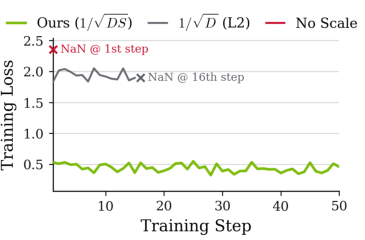
\includegraphics[width=0.95\linewidth]{figures/loss-vs-scale.pdf}
    \vspace{-3pt}
    \captionof{figure}{Training stability ablation.}
    \label{fig:gdn-key-scaling}
  \end{minipage}
\end{figure}
